\section{Source and target blockchains}

In the setting of sidechains, we wish to transfer assets from one blockchain to
another and then back. When assets can be transferred from one blockchain to
another but not back, we call it a \emph{one-way peg}. If assets can also be
moved back, we call it a \emph{two-way peg}. In each individual transfer of an
asset, we have a particular \emph{source blockchain}, from which the asset is
moved, and a particular \emph{target blockchain}, to which the asset is moved.
In a sidechain setting of two blockchains that are two-way pegged, both
blockchains can function as a source and a target blockchain for different
transfers.

While the motivation for the construction is to be able to move assets from one
blockchain to another, we wish to generalize the notion of sidechains from this
strict setting. In general, we would like the target blockchain to be able to
react to any \emph{event} that can occur on the source blockchain. Events within
a blockchain are any conditions to which local (to the particular blockchain)
smart contracts can react. For example, such events can be the fact that a
transaction with a particular \textsc{txid} took place, that a certain account
was paid a certain amount of money, or that a particular smart contract was
instantiated. Our sidechain construction allows the target blockchain to react
to events on source blockchain events in its target blockchain smart contracts
in the same way that the source blockchain smart contracts can.

\begin{figure}
    \caption{The source blockchain, pictured at the top, fires an event which is
             included in the black block. The firing of the event is confirmed
             by being buried under $k_1$ blocks in the source blockchain. After
             sufficient confirmation, the target blockchain, pictured at the
             bottom, reacts to the event with an action which is included in the
             white block. The white block is subsequently confirmed by being
             buried under $k_2$ blocks.}
    \centering
    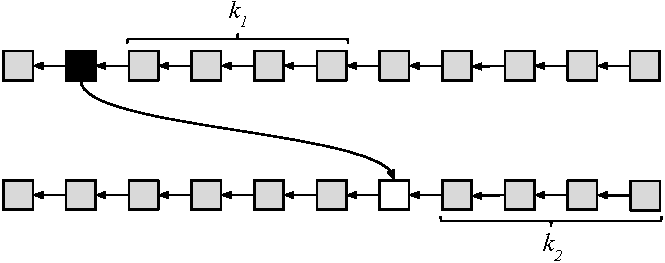
\includegraphics[width=0.9 \columnwidth,keepaspectratio]{figures/events.pdf}
    \label{fig.events}
\end{figure}
